\chapter{Аппаратура и условия наблюдений в эксперименте Конус-Винд} \label{chapt1}
Рассматриваемые в работе данные получены с помощью сцинтилляционного гамма-спектрометра 
Конус, предназначенного для изучения космических гамма-всплесков и установленного 
на космическом аппарате (КА) \textit{GGS-Wind}, лаборатории NASA по изучению 
солнечно-земных связей. КА был запущен в 1994 году на сложную высокоапогейную орбиту 
с удалением до двух миллионов километров от Земли. Подробное описание гамма-спектрометра 
Конус-Винд дано в работе~\citep{Aptekar1995SSR}.

Эксперимент Конус-Винд состоит из двух одинаковых NaI(Tl) сцинтилляционных 
гамма-спектрометров (S1 и S2), расположенных на противоположных сторонах 
стабилизированного вращением космического аппарата (КА) \textit{GGS-Wind}. 
Схематический вид КА \textit{GGS-Wind} и детектора приведён на рис.~\ref{img:KW_main_view}.
В настоящее время КА находится на орбите вокруг точки либрации $L_1$ 
на расстоянии около 1.5~миллионов километров от Земли. Оси полей зрения детекторов 
направлены в полюса эклиптики, при этом S1 направлен на южный полюс эклиптики, 
S2 на северный. Таким образом, обеспечивается обзор всей небесной сферы. 
Каждый детектор имеет эффективную площадь $\sim 80\textrm{--}160$~см$^2$ в 
зависимости от энергии падающего фотона и угла падения. Каждый детектор состоит 
из кристалла NaI(Tl) диаметром 13~см и высотой 7.5~см, помещенного в алюминиевый 
контейнер. Для снижения энергетического порога регистрации входные окна алюминиевых 
контейнеров кристаллов выполнены из бериллия. Кристалл просматривается фотоэлектронным 
умножителем (ФЭУ) через 20~мм свинцовое стекло, служащее для снижения фонового 
излучения от космического аппарата. Описанные параметры эксперимента дают 
возможность непрерывно производить наблюдения транзиентов, таких как гамма-всплески 
и мягкие гамма-репитеры, без затенения Землей и помех от радиационных поясов Земли 
в условиях исключительно стабильного фона. 

\begin{figure}[h]
  \begin{minipage}[h]{0.5\textwidth}
    \center{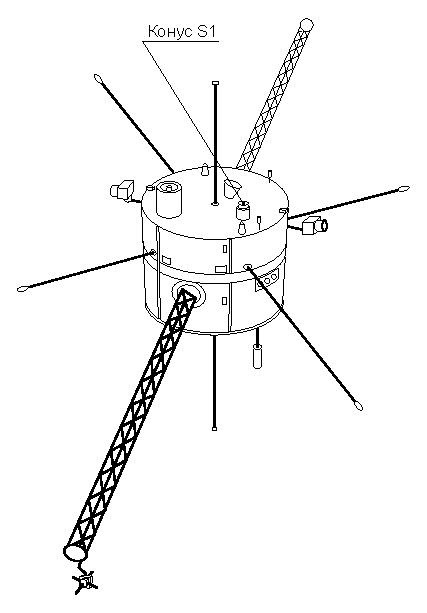
\includegraphics[width=1.0\textwidth]{wind-bw_v2} \\ а)}
  \end{minipage}
  \hfill
  \begin{minipage}[h]{0.5\textwidth}
    \center{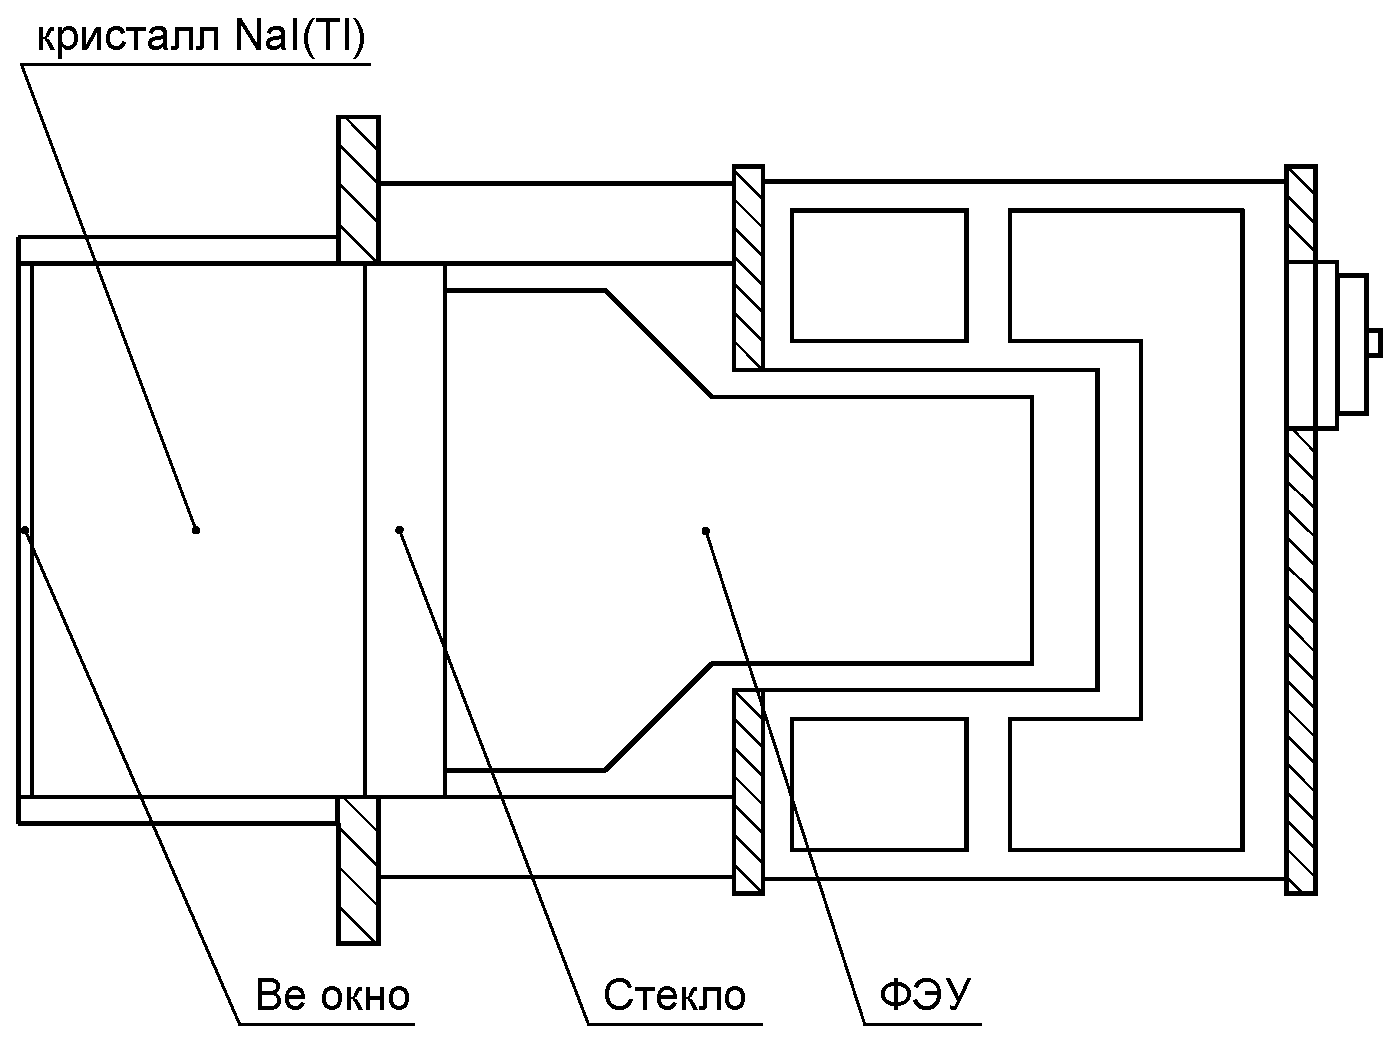
\includegraphics[width=1.0\textwidth]{detector_ru2} \\ б)}
  \end{minipage}
  \caption[Схематическое изображение КА \textit{GGS-Wind} и детектора Конус.]
  {Схематическое изображение КА \textit{GGS-Wind}~а) и детектора Конус~б).}
  \label{img:KW_main_view}  
\end{figure}

Два детектора работают независимо друг от друга в двух режимах наблюдений: 
фоновом и триггерном. Переход в триггерный режим происходит при статистически 
значимом превышении скорости счета над фоном $\approx 9 \sigma$, 
где $\sigma$~--- стандартное отклонение фона, на интервале 1~с или 140~мс 
в энергетическом диапазоне 50--200~кэВ. При этом скорость счёта фона 
определяется на предшествующем интервале длиной 30~с. В фоновом режиме ведется 
непрерывная запись временной истории в трёх каналах G1 (13--50~кэВ), G2 (50--200~кэВ) 
и G3 (200--760~кэВ) с временным разрешением 2.944~с. В триггерном режиме запись 
временной истории ведется в тех же энергетических каналах с временным разрешением 
от 2 до 256~мс в интервале от -512~мс до 229.632~с относительно времени срабатывания 
триггера.

Спектральные данные представляют собой 64 спектра, накопленных с разрешением от 64~мс до 8.192~с, 
которое автоматически выбирается в зависимости от интенсивности всплеска, 
в двух перекрывающихся энергетических диапазонах с установленными на Земле границами 
E1~(13--760~кэВ) и E2~(0.16--10)~МэВ. Изменения временного разрешения 
по ходу записи временной истории связаны с ограничениями на объем телеметрии, 
выделенной для эксперимента Конус. Результаты измерений записываются в оперативную 
память прибора. По окончании триггерного режима информация медленно переписывается 
в бортовую память, на что уходит 1--1.5~часа. На время перезаписи работа прибора 
в фоновом режиме прекращается. В это время резервирующая система продолжает измерения
скорости счета в окне G2 по каналу служебной телеметрии с разрешением 3.680~с.

\section{Функция отклика детектора}
Попадая в детектор, гамма-квант передаёт часть или всю свою энергию веществу 
сцинтиллятора, которая преобразуется в световую вспышку, регистрируемую ФЭУ. 
Заряд, собранный с анода ФЭУ, преобразуется в импульс напряжение, который усиливается и формируется для получения 
максимального соотношения сигнал-шум, после чего амплитуда импульса измеряется 
аналого-цифровым преобразователем (АЦП). В спектрометре Конус-Винд амплитуды импульсов 
измеряются двумя 64-х канальными АЦП, номинальные диапазоны которых 
соответствуют энергиям гамма-квантов 13--760~кэВ и 0.16--10~МэВ.

В общем виде исходный спектр излучения $f(E)$ связан с аппаратным спектром амплитуд 
импульсов $C(i)$ соотношением:
\begin{equation}\label{eq:response}
    C(i)=\int_{0}^{\infty} f(E)G(E,i) dE \mbox{ ,}
\end{equation}
где $G(E,i)$~--- функция отклика детектора, которая описывает вероятность кванту 
с энергией $E$ дать отсчёт в канал с номером $i$. На практике интегрирование 
заменяют суммированием, для Конус-Винд функция отклика рассчитывается для 255 
значений энергии в диапазоне 5~кэВ--30~МэВ и 20 углов падения 
от 0$^\circ$ до~95$^\circ$ с шагом~5$^\circ$.

В общем случае невозможно получить исходный спектр $f(E)$, зная $C(i)$, из 
уравнения~\ref{eq:response}.  Эта проблема решается выбором физически обоснованной 
спектральной модели и её подгонкой, после прямой свёртки с функцией отклика детектора, 
к спектру отсчётов. Подгонка осуществляется методом минимизации
\begin{equation}\label{eq:chisq}
    \chi^2=\sum\limits_{i=1}^n(C(i)-C_M(i))^2/C(i) \mbox{ ,}
\end{equation}
где $C_M(i)$~--- число отсчетов в i-м канале, полученное свёрткой модели и функции отклика.

Расчёт матрицы отклика детектора можно разделить на три этапа: расчёт спектра 
потерь энергии методом Монте-Карло, умножение полученного спектра на функцию 
нелинейности световыхода кристалла NaI(Tl) и последующая свёртка спектра, 
поправленного на нелинейность световыхода с функцией энергетического разрешения 
детектора.

Подробное описание методики расчета матриц отклика детекторов методом Монте-Карло 
и используемых процедур восстановления фотонных спектров падающего излучения 
приведены в работе~\citep{Terekhov_1998AIPC}.

\section{Калибровка спектров}
Реальные границы энергетических диапазонов изменяются со временем в сторону 
увеличения нижнего порога энергий регистрируемых гамма-квантов, это  
связано с накоплением радиационных дефектов в кристалле NaI(Tl) под воздействием 
солнечных космических лучей деградацией фотокатода ФЭУ. Определить реальное значение 
границ диапазонов можно благодаря наличию в спектрах фоновых линий 186~кэВ, 511~кэВ и~1460~кэВ.

Линия 186~кэВ связана превращением изотопа $^{123}\textrm{I}$, образующегося в 
сцинтилляторе под действием космических лучей, в $^{123}\textrm{Te}$ посредством 
электронного захвата, $T_{1/2}=13$~часов. Ядро $^{123}\textrm{Te}$ образуется в 
возбужденном состоянии. Возбуждение с наибольшей вероятностью снимается излучением $\gamma$-кванта 
с энергией 159~кэВ. Заполнение вакансии на K-оболочке происходит с излучением 
рентгеновских K$_{\alpha}$ линий с энергиями $\approx 27$~кэВ.

Линия 511~кэВ связана с образованием пар в материалах космического аппарата 
фоновыми гамма-квантами с энергиями $>1022$~кэВ.

Наиболее интенсивная линия 1460~кэВ сопровождает распад радиоактивного 
изотопа $^{40}\textrm{K}$, содержащегося в стекле, соединяющим кристалл и ФЭУ. 
Изотоп имеет два канала распада $\beta^{-}$ в $^{40}\textrm{Ca}$ с 
вероятностью 89.3\% и электронный захват в $^{40}\textrm{Ar}$ с вероятностью 10.7\%. 
Время полураспада $T_{1/2}=1.2\times10^9$ лет. Ядро $^{40}\textrm{Ar}$ образуется в
возбужденном состоянии. Возбуждение, с наибольшей вероятностью, снимается 
излучением гамма-кванта с энергией 1460~кэВ.

Для автоматической калибровки спектров автором настоящей работы была 
разработана процедура поиска и аппроксимации линии 1460~кэВ в аппаратных спектрах 
Конус-Винд. Положение границ диапазона E2 определялось непосредственно по положению 
линии 1460~кэВ. Положение границ E1 определялось по перекрытию с диапазоном E2, 
таким образом чтобы спектр отсчётов в E1 наилучшим образом соответствовал спектру в E2 
на основании статистики $\chi^2$. Разработанный метод позволяет получать калибровки 
для большинства регистрируемых всплесков.

Изменение границ энергетического диапазона Конус-Винд со временем представлено 
на рис.~\ref{img:KW_E_boundaries}. Резкие изменения границ в 1994--1996 годах 
связаны с изменением коэффициента усиления по команде с Земли. Дальнейший сдвиг 
границ диапазонов связан с деградацией кристалла и фотокатода ФЭУ под действием 
космических лучей. Скачкообразные изменения границ с последующей релаксацией 
к предшествующему тренду связаны потоками протонов высоких энергий, ускоренных в мощных 
солнечных вспышках класса "X"\ (см.~рис.~\ref{img:KW_E_boundaries_features}~a). 
Годичные изменения границ диапазонов (рис.~\ref{img:KW_E_boundaries_features}~б) 
на $\approx 3$\% синхронны вариациями температуры детекторов при движении 
КА~\textit{Wind} по орбите вокруг Солнца, при этом наибольшее значение границ 
соответствует наименьшей температуре.

\begin{figure}[h]
  \begin{minipage}[h]{0.5\textwidth}
    \center{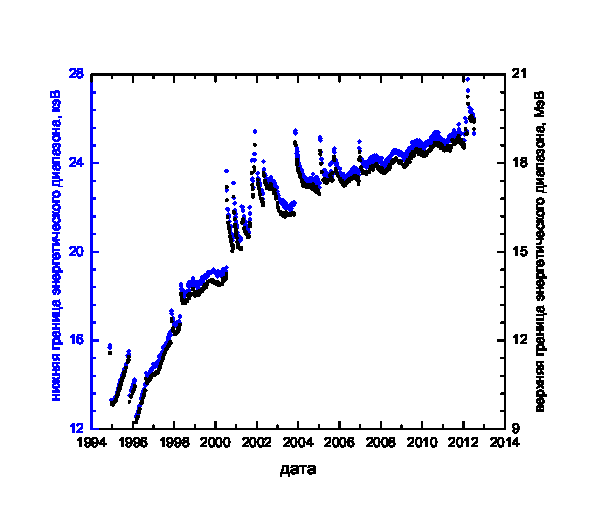
\includegraphics[width=1.0\textwidth]{gS1_calib} \\ а)}
  \end{minipage}
  \hfill
  \begin{minipage}[h]{0.5\textwidth}
    \center{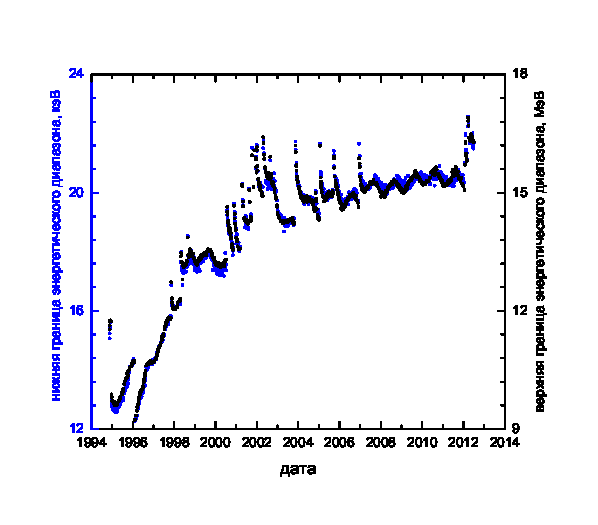
\includegraphics[width=1.0\textwidth]{gS2_calib} \\ б)}
  \end{minipage}
  \caption[Изменение со временем границ энергетического диапазона для детектора S1 и~S2.]
  {Изменение со временем границ энергетического диапазона для детектора S1~(a) и~S2~(б).}
  \label{img:KW_E_boundaries}  
\end{figure}

\begin{figure}[h]
  \begin{minipage}[h]{0.5\textwidth}
    \center{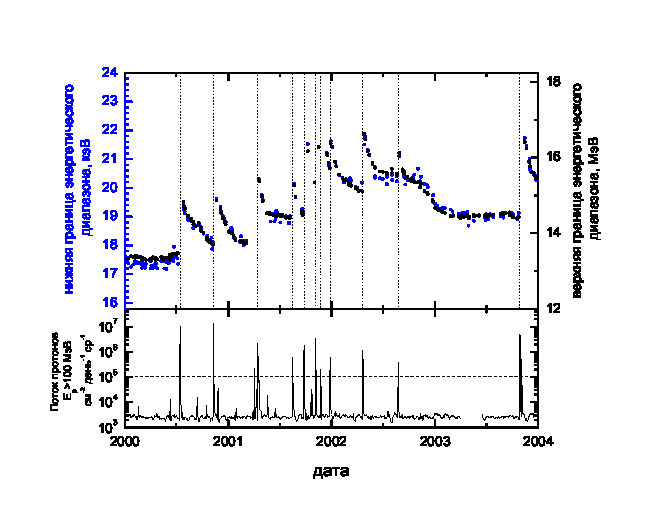
\includegraphics[width=1.0\textwidth]{gS2_protons_100MeV} \\ а)}
  \end{minipage}
  \hfill
  \begin{minipage}[h]{0.5\textwidth}
    \center{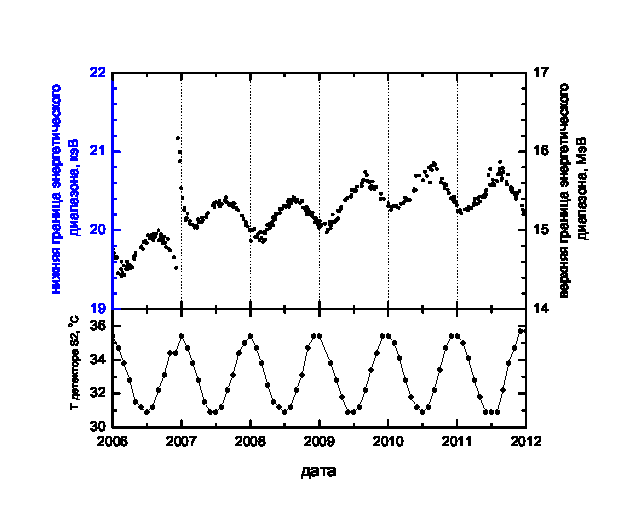
\includegraphics[width=1.0\textwidth]{gS2mE2_Temp} \\ б)}
  \end{minipage}
  \caption[Изменение со временем границ энергетического диапазона детектора S2 
  в 2000--2003~г и 2006--2011~г.]
  {Изменение со временем границ энергетического диапазона детектора S2. 
  Скачкообразные изменения границ диапазона в 2000--2003~г при облучении протонами с $E>100$~МэВ~(a). 
  Годичные изменения границ диапазонов в 2006--2011~г, связанные с вариацией температуры детекторов 
  при движении КА \textit{Wind} по орбите вокруг Солнца~(б).}
  \label{img:KW_E_boundaries_features}  
\end{figure}

\section{Чувствительность детекторов}
Под чувствительностью детектора понимается минимальный интегральный поток $S$~[эрг~см$^{-2}$], 
который вызовет превышение фона в канале детектора на заданном временном интервале 
на заданное число стандартных отклонений фона. При этом искомый поток будет зависеть 
от формы спектра падающего излучения и угла падения на детектор.

Уровень фона Конус-Винд благодаря нахождению прибора в межпланетном пространстве 
может оставаться постоянным на протяжении нескольких дней в периоды низкой 
солнечной активности. При анализе временных историй гамма-всплесков, 
зарегистрированных в триггерном режиме, фон аппроксимировался 
постоянным значением на интервале от $T_0 - 1000$~с до $T_0 - 250$~с, 
где $T_0$~--- время срабатывания триггера. Значительный отступ от триггерного 
времени связан с тем, что начало некоторых длинных всплесков лежит в предыстории. 

Уровни фона в трех диапазонах детекторов S1 и S2 незначительно различаются, 
что связано с различием границ диапазонов в детекторах. Скорости счёта фона 
на 2013~г равны для детектора S1: $\approx 950$~отсч~с$^{-1}$ в G1, 
$\approx 300$~отсч~с$^{-1}$ в G2, $\approx 150$~отсч~с$^{-1}$ в G3, 
для детектора S2: $\approx 1050$~отсч~с$^{-1}$ в G1, $\approx 350$~отсч~с$^{-1}$ в~G2, 
$\approx 130$~отсч~с$^{-1}$ в~G3. Ошибки скоростей счета фона на уровне $1 \sigma$ 
для всех детекторов равны: в G1 $\approx 1.3$~отсч~с$^{-1}$, в G2 $\approx 0.7$~отсч~с$^{-1}$, 
в G3 $\approx 0.5$~отсч~с$^{-1}$. 

Начиная с момента начала работы инструмента уровни фона медленно изменялись, 
что связано с изменением границ диапазонов со временем. Для детектора S1 относительное 
изменение фоновой скорости счёта составляет для G1 $\sim 17$\%, G2 $\sim 52$\%, G3 $\sim 38$\%. 
Для детектора S2 относительное изменение составляет для G1 $\sim 11$\%, G2 $\sim 45$\%, G3 $\sim 29$\%. 
В периоды повышенной солнечной активности наблюдались сильные кратковременные вариации фона. 
Изменение уровней фона представлено на рис.~\ref{img:KW_bg_drift}.

\begin{figure}[h]
  \begin{minipage}[h]{0.5\textwidth}
    \center{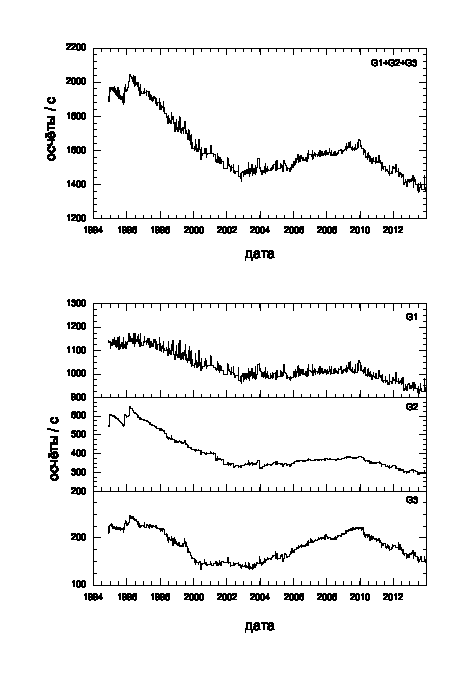
\includegraphics[width=1.0\textwidth]{gS1bg_cleaned} \\ а)}
  \end{minipage}
  \hfill
  \begin{minipage}[h]{0.5\textwidth}
    \center{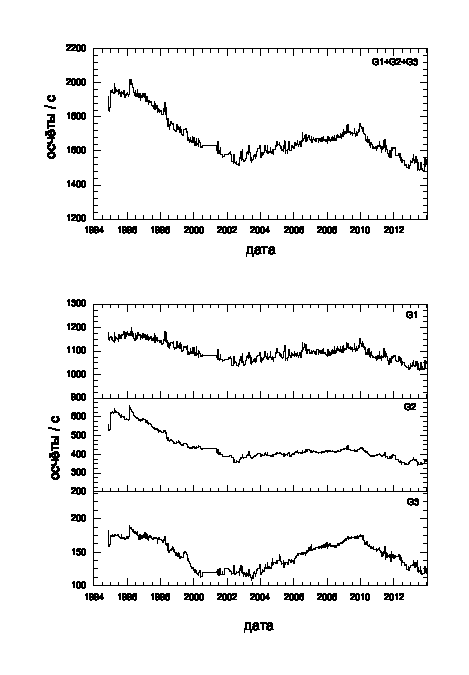
\includegraphics[width=1.0\textwidth]{gS2bg_cleaned} \\ б)}
  \end{minipage}
  \caption[Изменение со временем уровней фона детекторов S1 и~S2]
  {Изменение со временем уровней фона детекторов S1 а) и~S2 б). 
  Кратковременные повышения фона, связанные с потоками частиц от солнца удалены.}
  \label{img:KW_bg_drift}  
\end{figure}

Зная уровень фона, форму спектра можно вычислить интегральный поток, который 
даст превышение в $k\sigma$ над фоном на интервале $dT$.

Для расчёта $S$ использовались две функции, широко применяемые для моделирования 
спектров гамма-всплесков: степень с экспоненциальным обрезанием (сutoff power law, CPL)
\begin{equation}\label{eq:CPL}
\frac{dN}{dE} = A \left(\frac{E}{E_n}\right)^\alpha \exp\left(-\frac{E}{E_0}\right) \mbox{ ,}
\end{equation}
где A~--- амплитуда [фотоны см$^{-2}$~с$^{-1}$], $\alpha$~--- показатель степени,
$E_0$~--- энергия обрезания спектра, $E_n = 100$~кэВ~--- нормировочная энергия
и модель Банда (Band)~\citep{Band_1993ApJ}
\begin{equation}\label{eq:Band}
\frac{dN}{dE}=A \left\{
\begin{array}{lr}
\left(\frac{E}{E_n}\right)^\alpha \exp\left(-\frac{E}{E_0}\right) \mbox{, } 
&\mbox{если } E<(\alpha-\beta)E_0\\
\left(\frac{E}{E_n}\right)^\beta 
\left[(\alpha-\beta)\left(\frac{E_0}{E_n}\right)\right]^{(\alpha-\beta)} 
\exp(\beta-\alpha)  \mbox{, } &\mbox{если } E\geq(\alpha-\beta)E_0 \\
\end{array}
\right. \mbox{ ,}
\end{equation}
здесь $\beta$~--- показатель степени в области больших энергий, 
характерное значение которого $\beta = -2.5$. Энергия, на которую 
приходится максимум в спектре $E F_E = E^2 dN/dE$ равна $E_p=(\alpha+2) E_0$.

Для заданных спектральных параметров и единичной амплитуды вычислялся поток $F$~[эрг~см$^{-2}$~с$^{-1}$]
\begin{equation}\label{eq:flux}
F = \int_{E_{min}}^{E_{max}} E \left(\frac{dN}{dE}\right) dE
\end{equation}
и по этой же модели вычислялась скорость счёта $R$ в заданном канале путём свёртки 
спектра с трёх канальной матрицей отклика. Интегральный поток, который даст 
превышение в $k\sigma$ над фоном на интервале $dT$ вычислялся по формуле $S = k (F/R) \sqrt{R_{bg} dT}$, 
где $R_{bg}$~--- фоновая скорость счёта в канале. Формула представляет собой простой 
пересчёт порогового числа отсчётов в интегральный поток.

Зависимость интегрального потока $S$ для $k=9$ и $dT=1$~c от параметров спектральных 
моделей показаны на рис.~\ref{img:KW_min_fluence}. Расчёт $S$ был проведён для уровней фона 
$R_{bg}$: 1000~отсч~с$^{-1}$ для~G1, 350~отсч~с$^{-1}$ для~G2 и 150~отсч~с$^{-1}$ для~G3, 
и границ каналов G1 (20--80~кэВ), G2 (80--300~кэВ), G3 (300--1200~кэВ) 
близких к текущим значениям, и угла падения на детектор 60$^{\circ}$. 

Для канала G2, на основании которого вырабатывается триггер, модель Банда даёт 
\begin{equation}\label{eq:KW_Smin}
S\mbox{(20~кэВ--10~МэВ)} \approx 1\times10^{-6}\left(\frac{k}{9}\right)
\left(\frac{R_{bg} dT}{350\mbox{ отсч/с } 1\mbox{ с}}\right)^{1/2}\mbox{ эрг~см}^{-2}\mbox{ ,}
\end{equation}
где $k$~--- значимость детектирования в $\sigma$,
для всплесков с $E_p \lesssim 500$~кэВ. Для всплесков, чей спектр описывается 
моделью CPL (без степенного "хвоста") подобная чувствительность достигается в диапазоне $30\lesssim E_p \lesssim 800$~кэВ.
Для короткого триггерного интервала 140~мс и $k=9$ порог составляет $\approx 4\times10^{-7}$~эрг~см$^{-2}$

%Результаты расчётов были применены для расчётов верхних пределов на потоки гамма-излучения 
%от близкой сверхновой SN~2011fe типа Ia в галактике M101 на расстоянии 6.4~Мпк~\citep{Margutti_2012ApJ}.
%В статье взят порог GBM цитата "We therefore conclude that there is no statistically
%significant evidence for a SN-associated burst down to the
%Fermi-GBM threshold (fluence 4*10^−8 erg cm^−2 in the 8–1000 keV band)

\begin{figure}[h]
  \begin{minipage}[h]{0.5\textwidth}
    \center{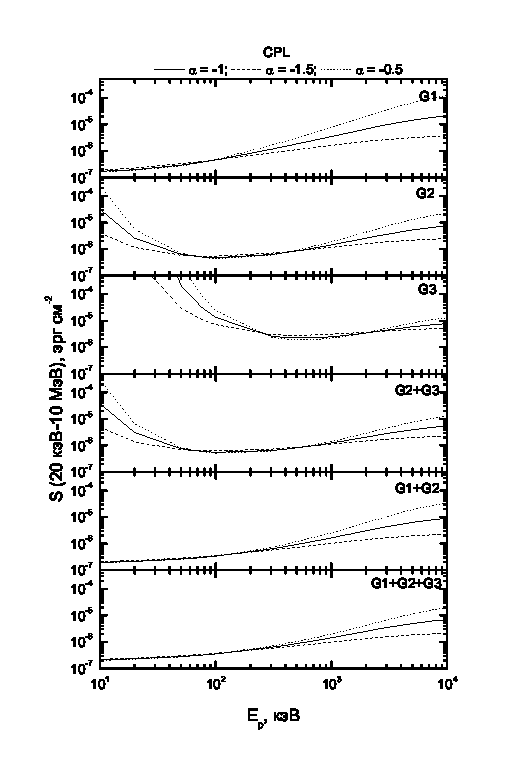
\includegraphics[width=1.0\textwidth]{gFluence_6ch_CPLru} \\ а)}
  \end{minipage}
  \hfill
  \begin{minipage}[h]{0.5\textwidth}
    \center{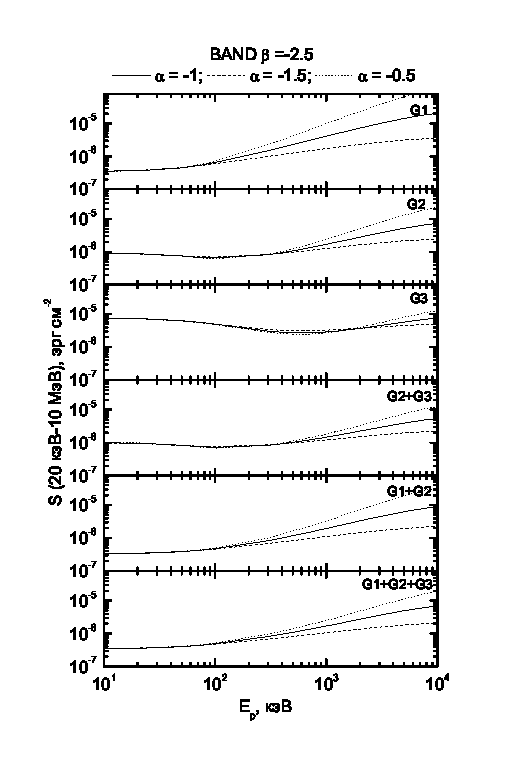
\includegraphics[width=1.0\textwidth]{gFluence_6ch_Bandru} \\ б)}
  \end{minipage}
  \caption[Минимальные регистрируемые интегральные потоки в диапазоне 20~кэВ--10~МэВ.]
  {Минимальные интегральные потоки в диапазоне 20~кэВ--10~МэВ, необходимые для детектирования 
  всплеска на уровне значимости $9\sigma$ для спектральной модели CPL с 
  показателями степеней $\alpha=-0.5$, $\alpha=-1$ и $\alpha=-1.5$~а) и~модели Band с теми же значениями $\alpha$ и $\beta=-2.5$~б).}
  \label{img:KW_min_fluence}  
\end{figure}